
After starting metaOmics, 
the first page is the metaOmics setting page in Figure~\ref{fig:GUIsetting}.  
There are 4 tabs on top of the page: Setting, Preprocessing, Saved Data and Toolsets.
Below the 4 tabs, 
the first header is the session information.
{
\color{red}
Why do we need session information?
}
The second header is Directory for Saving Output Files.
By clicking $\ldots$,
user can set default working directory, in which all the meta-analysis results will be saved.
User can view their current working directory on the top right corner.
The third header is Toolsets,
here users can view if individual packages are installed.
If the packages are installed, there is a checked installed status.
Otherwise, users can install individual package by clicking install blue button.

\begin{figure}[H]
\begin{center}
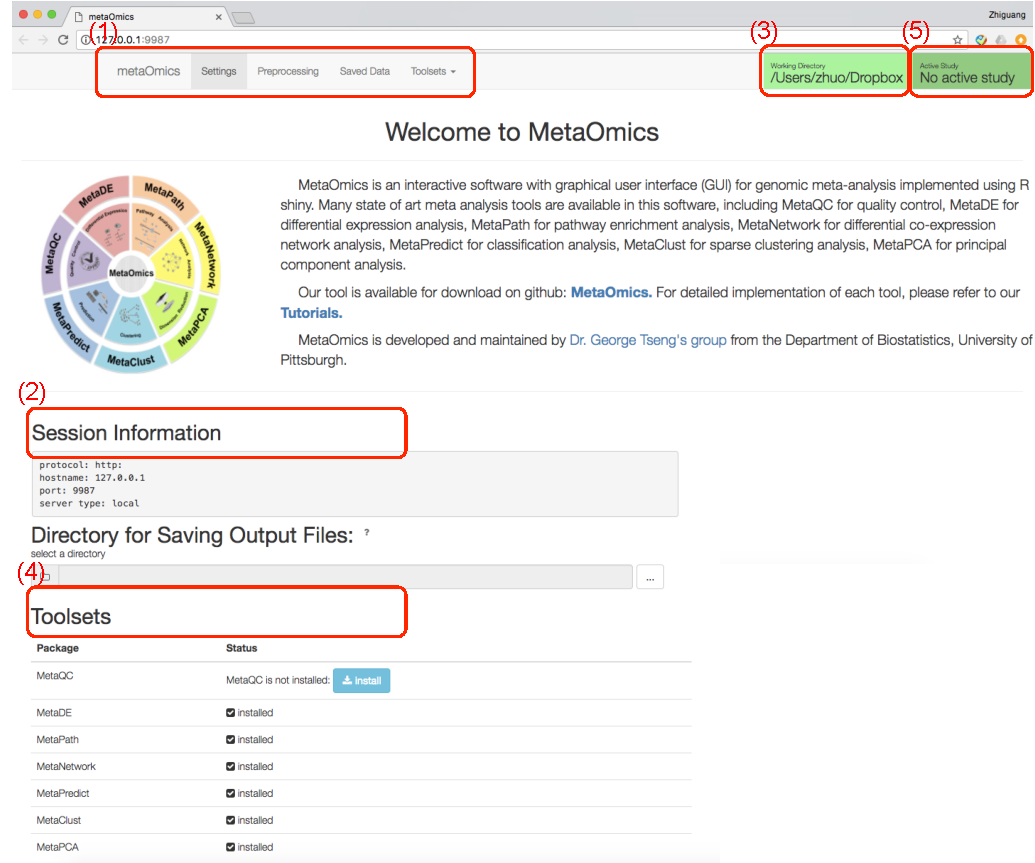
\includegraphics[scale=0.35]{./figure/preprocessing/GUIsetting}
\caption{GUI setting page}
\label{fig:GUIsetting}
\end{center}
\end{figure}

\subsection{Preprocessing}
\subsubsection{Uploading data}
If users go to the Preprocessing page as Figure~\ref{fig:GUIpreprocessing},
\begin{figure}[!htbp]
\begin{center}
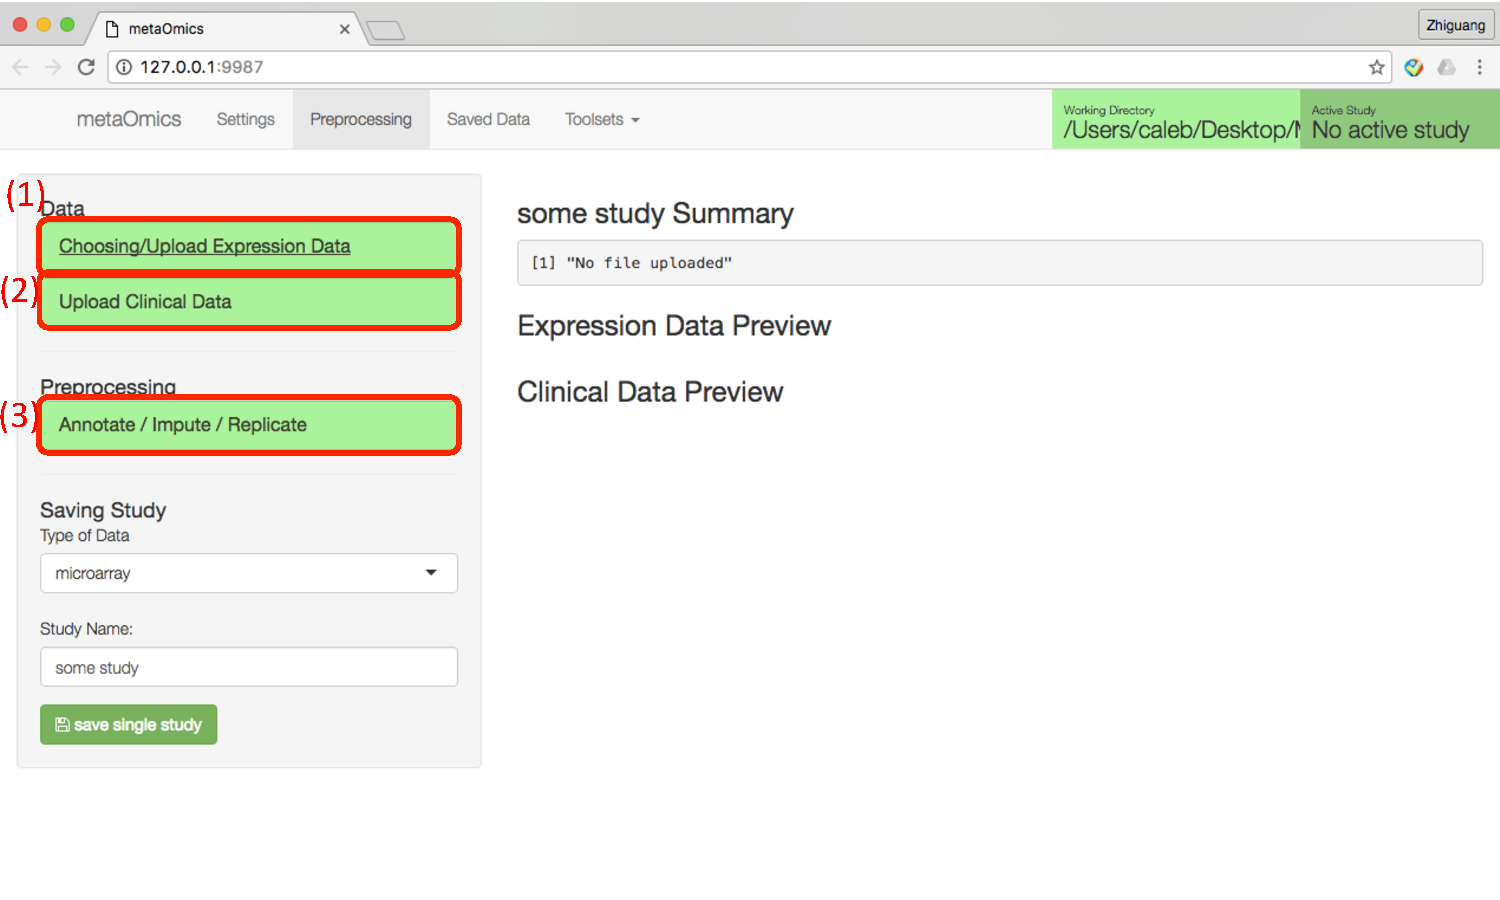
\includegraphics[scale=0.35]{./figure/preprocessing/GUIpreprocessing}
\caption{GUI Preprocessing page}
\label{fig:GUIpreprocessing}
\end{center}
\end{figure}
they are able to uploaded genomic data via the tab ``Choosing/Upload Expression Data".
The data should be prepared according to Section~\ref{sec:dataPrepare}.
Users may optionally upload Clinical Data, depending on biological purpose.
After uploading is complete,
users can preview their data on the right hand side of the page as Figure~\ref{fig:GUIpreview}.

\subsubsection{Preprocessing}
There are several expression data parsing option available on the left panel.
\begin{figure}[H]
\begin{center}
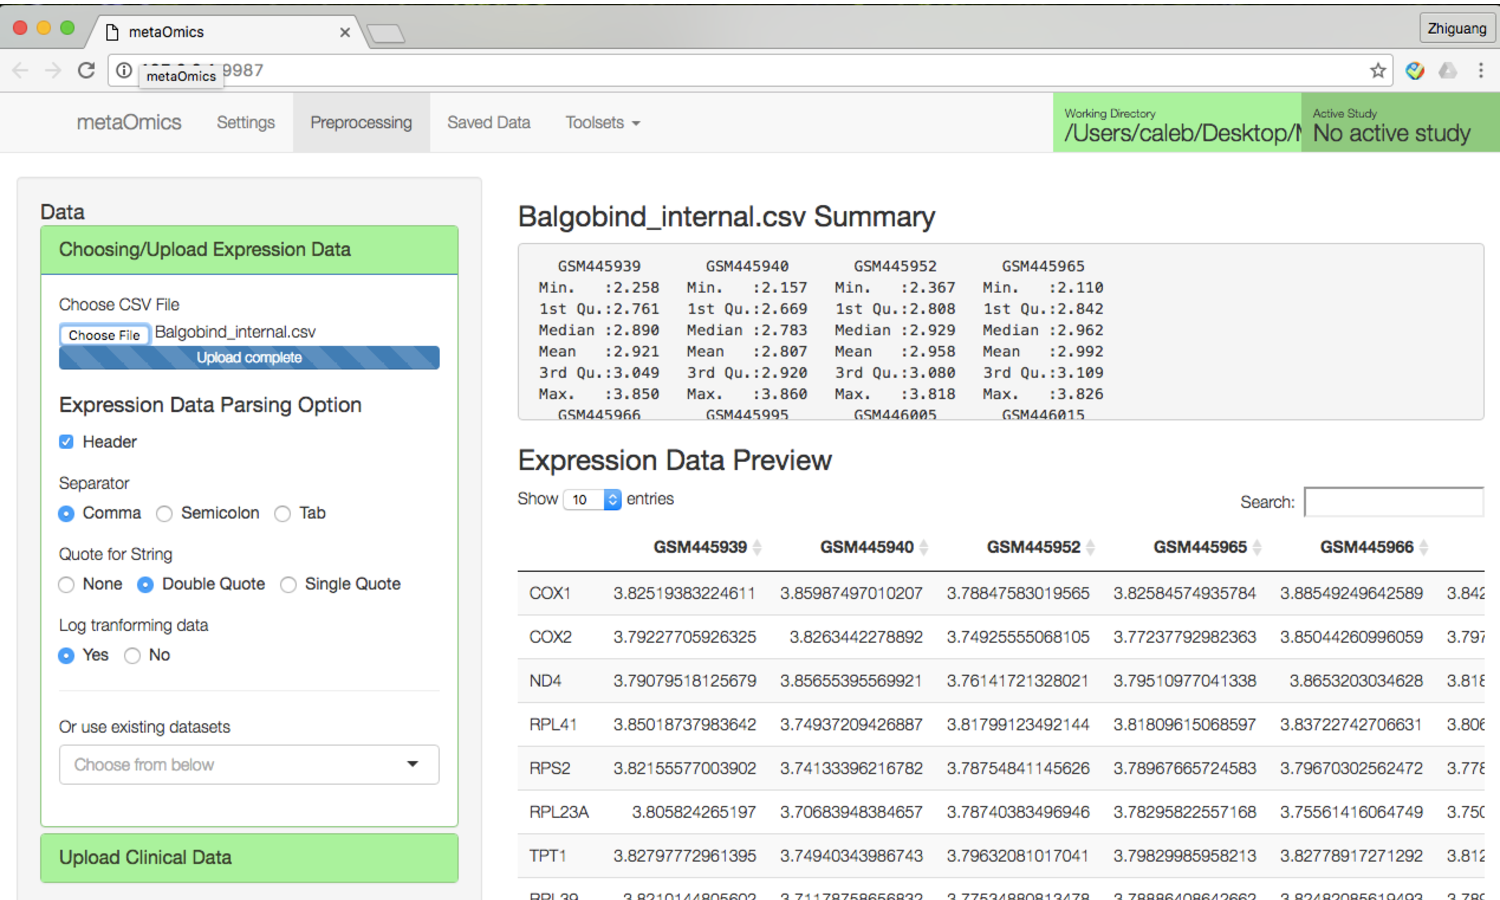
\includegraphics[scale=0.35]{./figure/preprocessing/GUIpreview}
\caption{GUI Preprocessing page}
\label{fig:GUIpreview}
\end{center}
\end{figure}
The MetaOmics suit also provide handlers for feature annotation, missing value imputation and multiple probe same genes.
Then users could specify type of data and study name.
Then click ``save single study" button, single study will be saved.

\subsubsection{Saved Data}
After uploading multiple studies w/o clinical data,
Users can turn to the Saved Data tab.
Users should select multiple datasets as Figure~\ref{fig:GUImerge}.
\begin{figure}[H]
\begin{center}
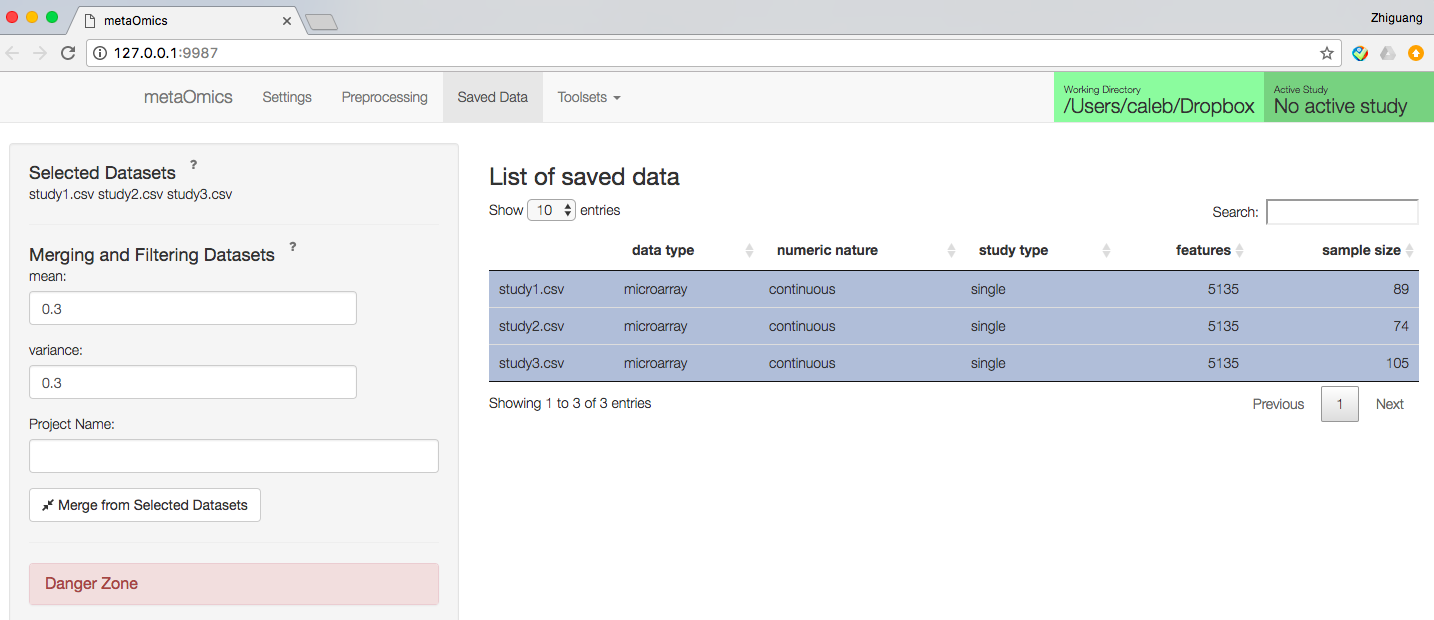
\includegraphics[scale=0.35]{./figure/preprocessing/GUImerge}
\caption{GUI Preprocessing page}
\label{fig:GUImerge}
\end{center}
\end{figure}
Users can select filtering criteria, enter merged study name and click on the Merge from Selected Datasets.
A merged dataset will appear on the left ``List of saved data" panel.
The last thing users need to do before using meta-analytic toolsets is select merged data and click on 
``Make merged Active Dataset" - A big green button.
Then the merged data becomes active study and shows up on the top right corner.
The active dataset serves as the input for all other MetaOmics modules.
